\newgeometry{%headsep=.5cm,footskip=.7cm,
lmargin=20mm,rmargin=20mm,tmargin=25mm,bottom=15mm}

\includegraphics[width=0.55\textwidth]{img/dariah-logo.png}
\vspace{20mm}
\maketitle
\vspace{5mm}
\begin{center}
\begin{LARGE}
\noindent\textbf{DARIAH-DE\\\vspace{3mm}Überführung~der~digitalen Forschungsinfrastrukturen~für~die e-Humanities~in~die Operational~Phase~(Betriebsphase)}
\end{LARGE}
\bigskip\bigskip
\vspace{10mm}

\begin{small}
\noindent Dieses Forschungs- und Entwicklungsprojekt wird / wurde mit Mitteln des Bundesministeriums für Bildung~und~Forschung~(BMBF), Förderkennzeichen 01UG1610A bis J, gefördert und vom Projektträger im Deutschen Zentrum für Luft- und Raumfahrt~(PT-DLR) betreut.\\
\end{small}
\vspace{20mm}

\includegraphics{img/bmbf.png}
\end{center}
\restoregeometry
\newpage
\normalsize
\begin{description}
\item[Projekt:] DARIAH-DE: Überführung der digitalen Forschungsinfrastrukturen für die e-Humanities in die Operational Phase (Betriebsphase)
\item[BMBF Förderkennzeichen:] 01UG1610A bis J
\item[Laufzeit:] März 2016 bis Februar 2019
\end{description}

\begin{description}
    \item[Dokumentstatus] Entwurf% or final
    \item[Verfügbarkeit] DARIAH-DE-intern
    \item[Autoren]
    \begin{itemize}
        \item[ ] % has to remain empty for formatting reasons
        \item[ ] N.\,N.
        \item[ ] N.\,N.
    \end{itemize}
\end{description}

\vspace{15mm}
\noindent\textbf{Revisionsverlauf:}\\
\begin{center}
    \begin{tabular}{l l l}
        Datum & Autor & Kommentare  \\
        30.11.2016 & N.N. & Vorlage 
    \end{tabular}
\end{center}



\vfill
\noindent\includegraphics[width=0.13\textwidth]{img/by.eps}

\noindent Dieses Werk ist unter einer Creative Commons Lizenz vom Typ Namensnennung 3.0 Deutschland zugänglich. Um eine Kopie dieser Lizenz einzusehen, konsultieren Sie http://creativecommons.org/licenses/by/3.0/de/ oder wenden Sie sich brieflich an Creative Commons, Postfach 1866, Mountain View, California, 94042, USA.
